\documentclass[11pt]{article}
\usepackage[margin=1.1in]{geometry}
\usepackage{amsmath,amssymb,amsthm}
\usepackage{hyperref}
\usepackage{booktabs}
\usepackage{array}
\usepackage[protrusion=true,expansion=false]{microtype}
\usepackage{xcolor}
\usepackage{enumitem}
\usepackage{titlesec}
\usepackage{tikz}
\usepackage{float}

\usetikzlibrary{arrows.meta,positioning,fit,shapes.geometric}

\hypersetup{colorlinks=true, linkcolor=blue!60!black, urlcolor=blue!60!black, citecolor=blue!60!black}

\titleformat{\section}{\large\bfseries}{\thesection.}{0.7em}{}
\titleformat{\subsection}{\normalsize\bfseries}{\thesubsection.}{0.6em}{}

\newcommand{\transcript}{\bigl(A_{1},A_{2},\textrm{PoKs},\textrm{ctxt},T,\sigma'_{A,P},R_{\cdot\cdot},s_{1},s_{2},e_{1},e_{2}\bigr)}

\newtheorem{theorem}{Theorem}
\newtheorem{definition}{Definition}
\newtheorem{remark}{Remark}
\newtheorem{lemma}{Lemma}
\newtheorem{observation}{Observation}
\usepackage[skip=0.6\baselineskip, indent=0pt]{parskip}
\title{\textbf{Babilonia: probabilistic coinjoin and covert betting}}
\author{waxwing}

\date{September 2026 \\ \medskip Version 2.0 (draft)}

\begin{document}
\maketitle

\tableofcontents

\section{Introduction}

There are essentially two approaches to online privacy. The first is \emph{uniformity}, probably best exemplified by mixnets \cite{chaum1981} but also seen in most other serious attempts to create privacy: they usually involve coordination by a central entity and require the actors in the system to behave identically or near-identically. A good example is the equal-output coinjoin design exemplified by Samourai and Wasabi \cite{zerolink,wabisabi}. These approaches are attractive in enabling quantifiable anonymity sets.

There are numerous issues with this approach, from disadvantages with central coordination to fragility with respect to other participants non-uniform behavior and the one that is unlikely to be captured in academic analysis:

\begin{quote}
Recognizably privacy seeking behavior is societally disadvantaged.
\end{quote}

That last point more than anything leads to a search for techniques in which privacy is a \emph{secondary} goal. This is not to make the fallacious claim that ``anonymity sets are larger when you don't choose to prioritize privacy''; this is trivially false, because standard activities (such as payments) don't have indistinguishable behaviour between parties. The idea is subtler, and is our ``second approach'': instead of trying to create an unambiguous, quantifiable anonymity set, the user simply creates (intentionally or not) alternative plausible intentions for their actions. Note how this defends against a different attacker: to defend against an adversary who targets your ownership, you should obscure ownership. To defend against an attacker who targets behavior, you should obscure behavior. Both attackers could be a threat to your personal well-being. This ties back to ``societally disadvantaged''.

For example, using Lightning \cite{lightning} to buy coffee may have the intention of saving transaction fees or speeding up 'confirmation' but may create privacy as a byproduct. This line of reasoning has been, and should continue to be, researched and investigated (and indeed the Lightning case nicely illustrates that you generally will defend against the former attacker \emph{as well as} the latter, that is, you will often obscure ownership too, at least partly). This reduces the societal disadvantage of general Bitcoin usage. If one focuses on on-chain Bitcoin the situation is clearly less bright, but this paper investigates an angle that is somewhat similar to Payjoin \cite{payjoin}.

If we take coinjoins \cite{maxwell2013} as by definition onchain Bitcoin transactions in which there is more than one actor providing input funds, then Payjoins are a coinjoin variant in which a payment occurs, but here we propose a twist on that idea: in case the user does not actually want to spend money at a merchant's shop, but is either willing or desiring to \emph{gamble}\footnote{Such a user should note the work of Bachelier and Einstein on random walks... and read Appendix B}, a similar outcome can be created not only with a trusted merchant, but also with a completely unknown counterparty, \textbf{assuming a completely trustless fair bet is possible}. We will present here a protocol to do exactly that.

The same technique can be applied to private coinswaps \cite{coinswap}. Further development of that idea is deferred to other work.

If we want to create privacy against the second aforementioned type of attacker, that is one who targets behavior, then one could easily and correctly argue that \emph{any} gambling activity has the desired effect: chips cashed out via the casino are apparently ``winnings'', not outputs of mixing. This applies, e.g. to online bitcoin exchanges, etc. One could add any of a vast number of similar techniques, both online and offline. What is distinct here is that a \emph{trustless} form of gambling does not require a central point of failure, with all the concomitant risks: trust in the entity, hacking risk, network monitoring, transaction graph being not distributed, performance problems etc. etc.

Finally let's mention the steganographic aspect. First, as this author noted in a blog post from 2019 \cite{payjoinblog}, the specific most useful effect of payjoin is that through the steganographic nature of such transactions --- a deep confusion of CIOH-violating transactions with others makes blockchain analysis far less effective. Additionally, through a specific suggested mechanism here\footnote{BIP324 \cite{bip324} decoy packets; see Section~\ref{sec:netlayer}.}, though others exist, we can arrange for bet transaction negotiation to be completely unknown to anyone except the counterparties, and the onchain footprint to be indistinguishable from ordinary payments \emph{on the happy path}. We don't claim perfection in this regard, but interestingly we don't have to, \emph{if} a betting market of such bets already exists, the covertness of ``looks like a payment'' is only one of two layers of defense against a privacy adversary.

\subsection{The pot-sweetener incentive}
\label{sec:potsweet}

This feature is only briefly mentioned in the below protocol design (see Section~\ref{sec:sweetener}), but it may be very important in creating participation. One bettor could incentivize any other bettor to take part by constructing the transactions so that the payouts are skewed slightly in their favor. This could occur in cases where Alice is looking mainly for a privacy effect, and Bob is more interested in the actual bet, i.e. gambling. This does \emph{not} suffer from the same watermarking flaw as Joinmarket \cite{joinmarket} in the specific sense that it is analogous to a merchant offering a discount for paying via coinjoin (that is, it changes the effective payment amount without even revealing the exact nature of the payment, let alone the betting function).

\section{Earlier work}
\label{sec:motivation}

The first successful onchain gambling system was probably SatoshiDice \cite{satoshidice}. In this system there was not a claim of trustlessness, but instead of \emph{verifiable after-the-fact fairness}. Gamblers placed bets by paying to specific addresses owned by SatoshiDice, and could calculate after the fact (using blockchain-derived entropy; details and caveats omitted for brevity) whether they \emph{should} have won or lost, and match that calculation against the outcome that was provided to them by the central entity.

Because of the control of funds by the central entity, a covert ``looks like a typical payment'' property was not achieved (nor, of course claimed); at least, if the transaction graph as a whole is analyzed. Here we are referencing what was already pointed out in the Introduction: the CPOF has a multifaceted disadvantage from a privacy perspective.

Recent research by Kurbatov and later GTT (\cite{kurbatov2025oprand,gerhardt2026}) investigated whether a fair coin-flip could be emulated on Bitcoin without complex onchain contracting and fully peer to peer, because no trust is required by the two parties in advance.

With regards to the former, note that Kurbatov's starting idea is an analogy with a ``thimbles game'' (a.k.a. ``shell game'') in which the player must guess under which cup (or ``thimble'') the ball is placed. He used hashing to hide the dealer's choice and made use of the ability to derive pubkeys that are hidden in hashed addresses (e.g. segwit pay-to-pubkey-hash) at the time of spending, so that ``reveal pubkey'' is atomic with ``broadcast spend''. To convert this to a taproot setting, as we will do, we make use of adaptor signatures, though several other tweaks are needed.

When speaking of the later paper \cite{gerhardt2026}, it seems that it was motivated by the desire for the existence of probabilistic payments and swaps executed not only in onchain form but also over Lightning or perhaps similar second layers. We will discuss a little more about this paper in the next section, because it is a substantially more powerful construction that the one shown here. \emph{This} paper examines a concrete instantiation of the same general idea for \emph{onchain bets}, but with a different extra property: maintaining a certain kind of \emph{privacy profile}.

Explaining further: the lack of any onchain contracts in what we describe here, replaced with offchain interactions using zero knowledge proofs, allows instantiation of a protocol with a steganographic footprint, so that the transactions can be interpreted by the outside world as normal peer to peer payments, or bets, without any emphasis on the privacy effect created, that is, the obfuscation of ownership of the resulting funds.

\subsection{Collaborative transactions without balance preservation - interesting?}

To state the obvious, this represents a radical change in the design, when compared with earlier coinjoin ideas, because here there is not an assumption that parties do not randomly gain or lose money, but rather only an assumption that the transfer of funds is fair in the statistical sense, and verifiably so, even against an adversarial and unknown counterparty.

Let's consider the outcome of repeated games. Those not of a gambling bent or not familiar with random walks are likely unaware of the existing theory about this.

To avoid spamming up the paper with gambling theory, I'll write a short ``takeaways'' here and defer (a little) more detail to Appendix B.

If the bet is a large fraction of your balance, consistently, over many bets, that's a big problem: something called ``asymmetric leverage'' will \emph{almost inevitably} eat up your funds over time (not that you can't get lucky with a win streak of course, but there is a strong tendency to lose, which seems counterintuitive if each single bet is fair, right ...).

However this is easily avoided by simply betting small amounts, and by not altering bet size according to your current balance. Think, the ``payments'' you're making are only say $x$ sats, whether your balance is $20x$ or $200x$. This takes away the above effect; now your balance experiences a random walk, but doesn't drift downwards (except from paying network tx fees). You can imagine the volatility of your balance as comparable to what you might pay a coinjoin coordinator, except (a) it's statistical: you might even \emph{gain} rather than lose and (b) what you're paying for is very different: a string of various payjoin-like transactions that don't look like coinjoins and cannot be flagged as such.

The biggest problem with this framing is: if you want these transactions to literally have the same distribution as other payments that exist, they cannot realistically be pinned to only very dusty payments. This tension is real; probably the realistic scenario is ``mostly small, or very small, but randomly varying bet sizes''.

Is it a compelling idea for users? That seems debatable. The idea of ``pot sweeteners'' mentioned above may help. There are pros and cons.

But we emphasize again that, like payjoin, \textbf{these transactions break subset-sum analysis, and they look exactly like payments, because \underline{they are payments}}.





%% ============================================================
\section{The verifiable onchain coin-flip}
\label{sec:crypto}
%% ============================================================

Here we will describe how to make the trustless fair bet using cryptography. We follow on here from the reasoning of Kurbatov \cite{kurbatov2025oprand} and GTT \cite{gerhardt2026}, without retracing all the steps and arguments from those works in the interest of brevity.

However, it is briefly worth mentioning more about the latter.

\subsection{Comparison with GTT (2026) \cite{gerhardt2026}}

This comparison is important, because in the most normal reading, \cite{gerhardt2026} is a significantly more powerful construction than the one we describe here. The rough comparison is: that paper describes how to do fair lottery/random selection with arbitrarily small success probabilities over \emph{swap} transactions, not joins (which also naturally integrates into Lightning), whereas this construction is described for joins and, as presented, only with 2 outcomes; we'll briefly describe how it can be extended to $N$ outcomes, but $N$ is realistically restricted to very small amounts, as our communication is linear in $N$. So why is the construction described here interesting? To quote from \cite{gerhardt2026} :

\begin{quote}
On-chain cost and fees. A complete winning probabilistic swap execution involves exactly four on-chain
transactions: two funding transactions (one per party), one payment-claim transaction by the dealer, and
one reward-claim transaction by the party. Each transaction uses a standard locking script OR(pktmp , T, pk)
as defined in Figure 2, which requires only a single signature for the claim path and a timelock check
for the refund path. These scripts are already supported natively by Bitcoin and Litecoin Taproot via
OP\_CHECKSIG and OP\_CHECKLOCKTIMEVERIFY (BIP 65), and do not require any additional opcodes or custom
spending conditions beyond what standard atomic swaps already use [61]. Consequently, probabilistic swap
transactions have the same on-chain structure as ordinary script-path Taproot spends.
\end{quote}

The point is as much the structure, as the cost: 4 onchain transactions, \textbf{with exposed scripts}, does not create an ideal 2-party betting system if we want to have onchain patterns that look like payments. We'll see both in this section and later ones, that we can achieve a ``fair bet'' scenario with very lightweight ZKPs and only standard keypath spend taproot outputs, \emph{and} transaction structures indistinguishable from ordinary payments (in the happy path), \textbf{and only 2 onchain transactions, not 4}\footnote{it is more practical to call it 2.5 transactions, but theoretically it's 2}. If \emph{these} aspects of the design are not important, it is likely that \cite{gerhardt2026} is more interesting. Note that \cite{gerhardt2026} does use a specific additional cryptographic feature to achieve its goals, namely a certain form of OPRF \cite{oprf}. Note also that with more interaction, it should be possible for that construction to have ``overlay'' transactions to remove the onchain script footprint, too. The ZKPs are intrinsically more weighty than here, due to the nature of what is being proved (and to achieve the goal of arbitrarily small probabilities without linear communication blowup).

One more preamble: this section describes the mechanism and, at its end, the on-chain payment-shaping that gives the bets their covert footprint (Section~\ref{sec:pst}); the network-layer covert-communication and discovery options are deferred to Section~\ref{sec:netlayer}.

\subsection{An outline of the protocol}

Throughout, $\mathbb{G}=\langle G\rangle$ denotes the secp256k1 group of prime order $p$, and $\mathbb{F}_p$ its scalar field; $H(\cdot)$ is the BIP340 challenge hash.

Note, we'll be a little sloppy (read: inefficient) on exact order of events here; that is deferred to the next section (\S3.3). Here we'll focus on the causal flow.

If funds are deposited by both parties (henceforth: Alice as ``dealer'', initiating the bet, and Bob as ``player'', accepting the bet, but noting that there is no trust in the dealer) into a joint MuSig2 \cite{musig2,bip327} output, we must construct two outgoing transactions: a RefundTx and a PayoutTx, as alternative spending paths from what we will call $U_1$, the utxo owned by the MuSig. Write $P_A,P_B$ for Alice's and Bob's \emph{funding} keys, so that $U_1$'s scriptPubkey is a keypath-only taproot output for the aggregate $P_{\mathrm{agg}}=\mathrm{KeyAgg}(P_A,P_B)$.

Next, to start the actual protocol, Alice randomly generates $N$ secret values $a_1,\dots,a_N$ from the set of valid scalars in $\mathbb{F}_p$ where $p$ is the order of the secp256k1 group. She sends $A_i = a_i G,\ i \in \{1,\dots,N\}$ to Bob along with a PoK of each of these secret discrete logs using the vanilla method (Schnorr signature). We call the $A_i$ the ``thimbles''. Here $N\ge 2$ is the number of thimbles: the game is \emph{$1$-of-$N$}, so an honest guess wins with probability $1/N$ and, for a fair game, is paid at odds $N{:}1$. The base case $N=2$ is the even-money coin-flip, and we carry it as the running example throughout; the general $1$-of-$N$ case is discussed in \S\ref{sec:nary}, and in the aggregated construction of \S\ref{sec:agg} different sub-bets use different $N$.

The RefundTx is straightforward: an \texttt{nLockTime} field, value $T_R$, is set in this transaction which prevents its spending before a certain time in the future; note that many wallets set \texttt{nLockTime} to a very recent block for anti-fee sniping \cite{antifeesniping}. $T_R$ will be set quite far out to ensure this backout is not possible until the contract completes.

This transaction RefundTx will reassign funds to their original owners and must be co-signed by Alice and Bob \emph{before the funding transaction is signed}.

Once the funding transaction is signed by both parties, the next stage is the provision, by Bob, of a receiving pubkey used in constructing the taproot scriptPubKey in the PayoutTransaction. This will take the form:

\[ K = W_b + A_y \]

The value $W_b = w_b G$ is a \emph{fresh hidden claim key} chosen by Bob, secret to this transaction and never revealed to Alice. We fix the index convention used throughout: $c\in\{1,\dots,N\}$ is \emph{Alice's} secret choice, and $y\in\{1,\dots,N\}$ is \emph{Bob's} secret guess; Bob wins iff $y=c$. So $A_y$ is the thimble corresponding to Bob's guess. His inability to know Alice's choice $c$ is clearly not dependent on any assumption cryptographically, only on Alice's general security.

Bob will have to attach a proof of honest construction of this value $K$, which is a simple $\Sigma$-protocol. This will be called $\pi_B$.

\begin{definition}[$\pi_B$: honest construction of the claim key]
\label{def:piB}
Given public thimbles $A_1,\dots,A_N\in\mathbb{G}$ and Bob's claim key $K\in\mathbb{G}$, $\pi_B$ is a zero-knowledge proof for the relation
\[
\mathcal{R}_{\pi_B}=\Big\{\ \big((K,A_1,\dots,A_N);\,(w_b,y)\big)\ :\ y\in\{1,\dots,N\},\ \ K = w_b\,G + A_y\ \Big\}.
\]
Equivalently, Bob knows the discrete log of $K-A_y$ with respect to $G$ for one branch $y$ (his guess), \emph{without revealing which}. It is realised as a $1$-of-$N$ CDS disjunction \cite{cds} of Schnorr proofs of knowledge of $\mathrm{dlog}_G(K-A_i)$ for some $i\in\{1,\dots,N\}$: soundness forces $K$ to equal one of the $A_i$ offset by a value Bob knows, and witness-indistinguishability hides $y$.
\end{definition}

Once Alice has verified $\pi_B$ she is ready to prepare the PayoutTx template; it has one input $U_1$, and at least one output, paying to a scriptPubkey, which we will call $O_K$, whose taproot internal key is $K$, and which has one leaf: a relative-timelock reclaim path for Alice, of the form
\[
\texttt{<}\,T_1\,\texttt{>}\ \ \texttt{OP\_CHECKSEQUENCEVERIFY}\ \ \texttt{OP\_DROP}\ \ \texttt{<}\,P_A\,\texttt{>}\ \ \texttt{OP\_CHECKSIG},
\]
where $T_1$ is a relative timelock in blocks (BIP68). $T_1$ is small relative to $T_R$. Thus the honest winning Bob spends $O_K$ by the \emph{key path} under $K$ (an ordinary taproot payment, no script revealed), while Alice can reclaim after $T_1$ blocks via this single script leaf only if Bob never claims.

In a later section (\ref{sec:coop}) we show how we can preserve the ``payment-like'' characteristic of this transaction even when the logic of the betting game gives the payout to Alice, that is, Bob has guessed incorrectly ($y\neq c$). An important note upfront: taproot's design \cite{bip341} enforces that keypath-spends for cases where a script-path leaf exists are \emph{not} distinguishable, even after the payment occurs, from keypath-spends from scriptPubKeys where no script-path spend existed, under the assumption that the observer does not know the original internal key used in constructing the output. This is because even pure keypath scriptPubkeys use a dummy script path formed by $H_{TapTweak}(P)$, and $P$ cannot be extracted by the observer.

Other outputs on the transaction are needed (usually, exactly one) to make this a typical payment transaction pattern; the choice of this does not affect any aspect of the game's security. The mechanism for this is described later in this document (\ref{sec:pst}).

With the full template of PayoutTx created, the next step is for Alice and Bob to start a MuSig2 negotiation, using the prepared nonces $R_{i,j}$ (which can be sent well in advance) as according to the standard MuSig2 workflow. After the nonce preparation, Alice can next create an \emph{adaptor signature}, denoted $\sigma'$, and provide along with it an adaptor point $T$.

The concept is that there will be a ZKP $\pi_A$ that will prove that $T$'s discrete log $t$ is a kind of ``decryption secret'' that will allow Bob to calculate \emph{one of} $a_1, a_2$ and thus get the full private key of $K$, but he will not be able to deduce which, until the adaptor signature (or ``encrypted signature'' a la Fournier \cite{fournier}) is completed with the full signature, i.e. when the transaction is broadcast.

Notice a crucial game-theoretical aspect of this: the information hiding \textbf{has to work both ways}. This point was expanded on in some detail in GTT \cite{gerhardt2026}. If Alice could deduce anything about Bob's choice, encoded in $K$, she could choose to back out preferentially at this step of the protocol. And if Bob knew Alice's choice, he could do the same at the next step (when he co-signs). Because Alice \emph{doesn't} know Bob's choice at this step, while she \emph{could} still get cold feet and fall back to Refund, she has no more incentive to back out now, than she did at the start.

When Bob receives this adaptor, a ciphertext $\textrm{ctxt}$, and the corresponding zero knowledge proof $\pi_A$ (explained in a moment), he can verify the adaptor pre-signature:

\[\sigma' G \stackrel{?}{=} R_{A} - T + e\,\mu_A P_A,\qquad e = H\big(R_{\mathrm{agg}},\,P_{\mathrm{agg}},\,m_{\mathrm{payout}}\big),\]

\ldots where $R_{A}$ is Alice's contribution to the aggregate nonce $R_{\mathrm{agg}}$, and $\mu_A$ is Alice's MuSig2 key-aggregation coefficient (we write $\mu_A$, not $a_A$, to avoid clashing with the thimble scalars $a_1,a_2$); thus $\mu_A P_A$ is Alice's delinearized key component and $m_{\mathrm{payout}}$ is the PayoutTx sighash. The check holds because Alice's completed partial would satisfy $\sigma_A G = R_A + e\,\mu_A P_A$, and the adaptor partial is short by exactly $t$: $\sigma' = \sigma_A - t$, i.e. $\sigma'G = R_A - T + e\,\mu_A P_A$. See MuSig2 \cite{musig2,bip327} for the aggregation details, and \cite{fournier} for adaptor (one-time verifiably-encrypted) signatures.

Additionally, he of course must verify $\pi_A$:

\begin{definition}[$\pi_A$: well-formedness of the encrypted outcome]
\label{def:piA}
Fix a pad function $f:\mathbb{F}_p\to\mathbb{F}_p$ (the ``decryption'' map; concrete choices in Section~\ref{sec:pia}). Given public $(\textrm{ctxt},T,A_1,\dots,A_N)$ with $\textrm{ctxt}\in\mathbb{F}_p$ and $T,A_1,\dots,A_N\in\mathbb{G}$, $\pi_A$ is a zero-knowledge proof for
\[
\mathcal{R}_{\pi_A}=\Big\{\ \big((\textrm{ctxt},T,A_1,\dots,A_N);\,(t,c,a_c)\big)\ :\ c\in\{1,\dots,N\},\ \ T=tG,\ \ A_c=a_c G,\ \ \textrm{ctxt}=a_c+f(t)\ \Big\}.
\]
In words: the adaptor point $T$ has discrete log $t$; the ciphertext decrypts under the pad to a scalar $a_c$ whose public image $A_c$ is one of the $N$ published thimbles; and the branch $c$ (hence the outcome) is hidden.
\end{definition}

Note that we refer to a generic function $f$ acting on the secret value $t$; this, and the actual concrete instantiation of $\pi_A$, are discussed in Section~\ref{sec:pia}.

$\pi_A$ represents Bob's guarantee that when the adaptor is completed, he will be able to convert $\textrm{ctxt}$ into $a_c$, Alice's actually chosen discrete log, via the relation:

\[a_c = \textrm{ctxt} - f(t).\]

Once Bob has verified both the adaptor and the proof $\pi_A$, he is now safe that the bet is fair: he sends $\sigma_B$, which is his partial signature for the PayoutTx.

Once Alice receives $\sigma_B$, she is safe to broadcast the transaction, which:

\begin{itemize}
\item reveals $\sigma$, the total valid BIP340 signature on $U_1$;
\item which Bob sees, and he calculates $t = \sigma - \sigma_B - \sigma'$;
\item he then calculates $a_c = \textrm{ctxt} - f(t)$;
\item he then compares $W_b + a_c G$ with $K$; if it is the same, he has the secret key $w_b+a_c$ of $O_K$'s internal key and can spend by the key path;
\item if he does not spend before the relative timelock $T_1$, Alice spends via the CSV path, or uses a cooperative optimization --- see Section~\ref{sec:coop}.
\end{itemize}

\subsection{The protocol as a sequence of messages}

We assume that one peer has identified another candidate peer and there is a reliable transport via which to send messages in both directions. Alice is called the ``Dealer'' and Bob is called the ``Player''. The absolute timelock $T_R$ for the RefundTx must be much larger than the relative timelock $T_1$ for the PayoutTx's destination scriptPubKey so that the contract cannot be backed out of before its expiration.

\begin{enumerate}
\item Dealer sends funding information: $u_A$ for funding FundingTx, $P_A$ for MuSig2 destination key $M$ (will be outpoint $u_1$), receiving address for RefundTx $R_A$, change address for PayoutTx $C_A$, coop-overlay address $O_A$, nonces for RefundTx and PayoutTx and CoopOverlay signature negotiation. Simultaneously, she sends $A_1,\dots,A_N$ and a proof of knowledge of the dlogs $a_1,\dots,a_N$, keeping the latter secret.
\item Player validates the PoK of $A_1,\dots,A_N$. Player sends funding information: $u_B$ for funding FundingTx, $P_B$ for MuSig2 destination key $M$, (will be outpoint $u_1$), receiving address for RefundTx $R_B$, change address for PayoutTx $C_B$, nonces for RefundTx and PayoutTx and CoopOverlay signature negotiation, and $K$ for settlement transaction, along with a ZKP $\pi_B$ proving that $K$ is of the form $A_y + W_b$ for his choice $y$ from $A_1,\dots,A_N$ and a further key he proves knowledge of (see above for details).
\item Dealer validates $\pi_B$. Dealer calculates MuSig2 destination address $M$ and outpoint $u_1$, and full FundingTx ($u_A, u_B \rightarrow u_1, C_B$). Dealer then calculates RefundTx ($u_1 \rightarrow R_A, R_B$) and calculates partial sig on RefundTx $\sigma_{A,R}$. Sends $\sigma_{A,R}$.
\item Player calculates MuSig2 destination address $M$ and outpoint $u_1$, and full FundingTx ($u_A, u_B \rightarrow u_1, C_B$). Player then calculates RefundTx ($u_1 \rightarrow R_A, R_B$). Having received $\sigma_{A,R}$ he now calculates his own partial sig on RefundTx $\sigma_{B,R}$, and validates the full signature on RefundTx (if invalid, aborts). Sends $\sigma_{B,R}$.
\item Dealer validates that the RefundTx is fully signed; if not, aborts. She then calculates the adaptor signature and point $\sigma'_{A, P}, T$ for PayoutTx signing on $u_1$ (noting that the nonces were already exchanged for this MuSig session).   She then calculates $\pi_A$ and ciphertext $\textrm{ctxt}$ as described above and sends $\sigma'_{A, P}, T, \pi_A, \textrm{ctxt}$. $T$ was chosen so that $\textrm{ctxt} = a_c + f(t)\ \textrm{mod}\ p$ and $tG = T$ and $a_c \in \{a_1,\dots,a_N\}$ and $\pi_A$ proves this.
\item Player verifies $\sigma'_{A, P}, T, \pi_A$ against PayoutTx and the predetermined nonces. If it verifies, he calculates, and then sends $\sigma_{B,P}$.
\item Dealer signs the FundingTx (which she already calculated) on $u_A$ to get $\sigma{A, F}$ and passes this as a PSBT to Player.
\item Player co-signs the FundingTx (which he already calculated) on $u_B$ to get $\sigma_{B, F}$ and combines this with the PSBT to broadcast the FundingTx.
\item Both sides wait for confirmation of funding transaction. Note that they already have the PayoutTx, which is ($u_1 \rightarrow O_K, C_A$)
\item Dealer constructs fully signed PayoutTx, by calculating $\sigma_{A,P}$. She sends $t$ and her co-signature $\sigma_{A, O}$ on the CoopOverlayTx to the Player (but does \emph{not} broadcast PayoutTx).
\item Player sees $t$, and uses it to calculate $a_c = \textrm{ctxt} - f(t) \ \textrm{mod}\ p$. And then compares $a_c G$ with $A_y$, if they match, he has won and will calculate the full MuSig2 cosignature on PayoutTx as $\sigma_{B,P} + \sigma'_{A, P} + t$ and use it to broadcast PayoutTx. And must send another payment from $O_K$ to his own wallet independently before the timeout clause $T_1$.
\item If they do not match, he calculates CoopOverlayTx, and his co-signature $\sigma_{B,O}$ on that transaction, and broadcasts it (knowing he has lost the bet anyway, he does this to maintain a payment-shaped transaction).
\item In case the Player disappears and does not complete the previous step promptly, the Dealer broadcasts, PayoutTx which pays $u_1$ into an output she will control after $T_1$ blocks\footnote{The player can ``grief'' here also, by waiting for this event even if he won; but as noted elsewhere, this is not a money gaining attack, it only destroys a mild privacy effect for both participants}.
\end{enumerate}

In cases where the steps say ``X validates Y'', it is to be understood that if validation fails, that participant aborts, either by doing nothing, or, if they have already committed funds, by broadcasting RefundTx as is obvious according to context. Step 13 is a specific kind of abort; the bet completes, but some privacy w.r.t. outside observers is lost.

\subsection{The general $1$-of-$N$ game}
\label{sec:nary}

The even-money ($N=2$) game generalizes directly to $1$-of-$N$ for any small $N$, giving Bob win probability $1/N$ paid at odds $N{:}1$. Nothing in the construction is specific to $N=2$: Alice publishes $N$ thimbles $A_1,\dots,A_N$, and both $\pi_B$ (Definition~\ref{def:piB}) and $\pi_A$ (Definition~\ref{def:piA}) are already stated over $N$ branches. Each is realised as a $1$-of-$N$ CDS-OR (the $N=2$ instance is detailed in \S\ref{sec:squaring-proof}): one honest branch, plus $N-1$ simulated branches, whose sub-challenges sum to the Fiat--Shamir challenge, $\sum_{i=1}^{N} e_i = e \bmod p$. The security arguments are unchanged in form: knowledge-soundness is the same special-soundness extraction on whichever branch differs between two accepting transcripts, and branch-hiding rests on the same square-DDH assumption --- Appendix~A gives the reduction for $N=2$, and the $N$-branch case follows from it by a standard hybrid over the thimbles $A_i$.

The one real cost is communication: the sigma-protocol proofs are $O(N)$ in size, so this is practical only for small $N$ (a SNARK proving system, or the OPRF route of GTT \cite{gerhardt2026}, would remove the $O(N)$ blow-up). In practice this is not a binding limitation, because $N$ is deliberately kept small --- both to bound the dealer's fronted liquidity and because, as we show in \S\ref{sec:agg}, the covertness of the payout \emph{amount} comes not from large $N$ but from \emph{aggregating} many small-$N$ sub-bets. (A $k$-of-$N$ threshold variant is also possible but not pursued here.)

\subsection{Payment-shaped transactions}
\label{sec:pst}

There is no \textbf{requirement} for any privacy outcome here; the protocol functions purely as a wager. However it is noteworthy that the specific design above has an extremely minimal onchain footprint, and so it is \textbf{the cheapest as well as the most private}. This fits in with taproot's design principles (and indeed, offchain payments, also). So it is plausible that ordinary bets take this structure, even if the users don't care about privacy (see the Introduction).

But there is one specific privacy outcome that falls out of the root design:

\begin{quotation}
Because of the symmetrical safety/security of the cryptographic construct, a purely peer to peer protocol is possible. Because of \emph{that}, dual funding is not only possible, but natural. Because of \emph{that symmetry of roles}, a partial breakage of common input ownership heuristics \cite{fistful} is inevitable. Because of \emph{that}, this protocol has a natural privacy effect, though not a very strong one on a per-transaction basis (much stronger over the whole transaction graph of bets).
\end{quotation}

Shooting for a stronger privacy effect than that is possible but it isn't necessary. The on-chain half of that stronger effect --- making the bet transactions read as ordinary payments --- is described here; the network-layer half (covert negotiation and discovery) is deferred to Section~\ref{sec:netlayer}.

The other thing needed for the ``first layer defence'' of having these bets look like normal payments, is to disguise the fact that cooperation is occurring (because in fact, that is the sense in which they are not normal payments --- they \emph{are} payments, the only thing different is that they are co-funded, which breaks CIOH).

The PayoutTx spends a single input $U_1$ (it can optionally spend more but that's more complex) to a standard P2TR destination. It should also have a change output, which it naturally doesn't have.

The FundingTx has a different-shaped problem: its default structure has each party contribute one or more inputs, and the output $U_1$ is then accompanied by \emph{two} change outputs. This is far from ideal, as 3-output transactions are far from common; we want a two-output transaction. The natural way to achieve this is for the dealer to provide a utxo which is equal to their suggested bet size (optionally, the player could do the same); this way they have no change output. But that is very restricting.

Fortunately, both problems are resolved by one idea: \textbf{spread the two change outputs across the two transactions}. The dealer (Alice) contributes her \emph{entire} input to the pot and takes no change in the funding transaction; her change is instead released as the second output of the PayoutTx. The player (Bob) takes his change in the funding transaction as usual. Writing $F_A, F_B$ for the two funding inputs, $a,b$ for the (equal) stakes, $S = a+b$ for the at-risk pot, and $c_A = F_A - a$, $c_B = F_B - b$ for the two change amounts, the pot is $U_1 = F_A + b = S + c_A$.

The choice of \emph{which} change goes in \emph{which} transaction is deliberate. The Bob-wins branch must complete \textbf{without any cooperation from Alice} (she has no incentive to help a winning counterparty), so we want that branch to have the payment-like two-output shape \emph{automatically}. Because Alice's change is an output of the \emph{pre-signed} settlement, the Bob-wins settlement is two-output regardless of the outcome and regardless of cooperation (Figure~\ref{fig:bobwins}); Bob then spends his claim output $O_K$ by an ordinary key path. The Alice-wins branch (Figure~\ref{fig:alicewins}) is the cooperative key-path spend of Section~\ref{sec:coop}, which the parties are jointly motivated to use.

\begin{figure}[h]
\centering
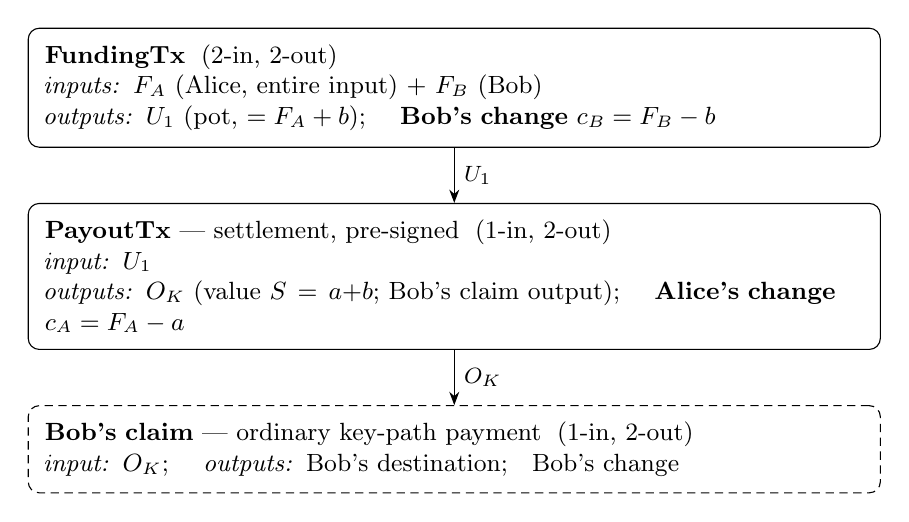
\begin{tikzpicture}[>=Stealth,
  tx/.style={draw, rounded corners, align=left, inner sep=6pt, font=\small, text width=10.4cm},
  ann/.style={font=\footnotesize}]
\node[tx] (f1) {\textbf{FundingTx} \;(2-in, 2-out)\\
  \emph{inputs:} $F_A$ (Alice, entire input) $+$ $F_B$ (Bob)\\
  \emph{outputs:} $U_1$ (pot, $= F_A + b$); \quad \textbf{Bob's change} $c_B = F_B - b$};
\node[tx, below=7mm of f1] (p1) {\textbf{PayoutTx} --- settlement, pre-signed \;(1-in, 2-out)\\
  \emph{input:} $U_1$\\
  \emph{outputs:} $O_K$ (value $S = a{+}b$; Bob's claim output); \quad \textbf{Alice's change} $c_A = F_A - a$};
\node[tx, below=7mm of p1, densely dashed] (c1) {\textbf{Bob's claim} --- ordinary key-path payment \;(1-in, 2-out)\\
  \emph{input:} $O_K$; \quad \emph{outputs:} Bob's destination; \; Bob's change};
\draw[->] (f1) -- (p1) node[midway, right, ann] {$U_1$};
\draw[->] (p1) -- (c1) node[midway, right, ann] {$O_K$};
\end{tikzpicture}
\caption{\textbf{Bob wins.} Alice's change rides in the pre-signed settlement, so that transaction is two-output automatically --- no cooperation from Alice required. Every transaction has the dominant two-output shape.}
\label{fig:bobwins}
\end{figure}

\begin{figure}[h]
\centering
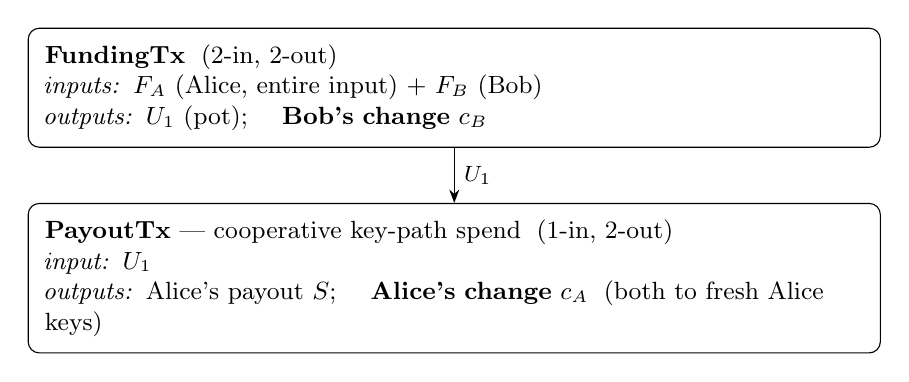
\begin{tikzpicture}[>=Stealth,
  tx/.style={draw, rounded corners, align=left, inner sep=6pt, font=\small, text width=10.4cm},
  ann/.style={font=\footnotesize}]
\node[tx] (f2) {\textbf{FundingTx} \;(2-in, 2-out)\\
  \emph{inputs:} $F_A$ (Alice, entire input) $+$ $F_B$ (Bob)\\
  \emph{outputs:} $U_1$ (pot); \quad \textbf{Bob's change} $c_B$};
\node[tx, below=7mm of f2] (p2) {\textbf{PayoutTx} --- cooperative key-path spend \;(1-in, 2-out)\\
  \emph{input:} $U_1$\\
  \emph{outputs:} Alice's payout $S$; \quad \textbf{Alice's change} $c_A$ \;(both to fresh Alice keys)};
\draw[->] (f2) -- (p2) node[midway, right, ann] {$U_1$};
\end{tikzpicture}
\caption{\textbf{Alice wins.} Rather than the settlement (which would force a script-path reclaim of $O_K$), the parties co-sign a single key-path spend of $U_1$; Alice's two outputs go to fresh keys and read as payment $+$ change.}
\label{fig:alicewins}
\end{figure}

In this way, both Alice and Bob receive a change output from the execution of the protocol, unconditionally whether they won or lost the bet, and all the ``happy-path'' transactions have the two-output profile that is dominant in the distribution of onchain transactions, achieving the covertness property desired.

We note also the somewhat trivial points that nLockTime and nSequence should align with typical network behavior.

\subsection{A pot-sweetener example}
\label{sec:sweetener}

To illustrate the idea from Section~\ref{sec:potsweet}, we show a case of Alice, the dealer, incentivizing Bob, the player. Alice starts with a utxo of size 0.2 and Bob with one of 0.8. Alice decides that the pot contributions should be size 0.05, but she also adds a sweetener of 0.01 for Bob to slightly favor him. Then we have:

% Requires in preamble:  \usepackage{tikz}  \usetikzlibrary{arrows.meta}
\begin{figure}[H]
\centering
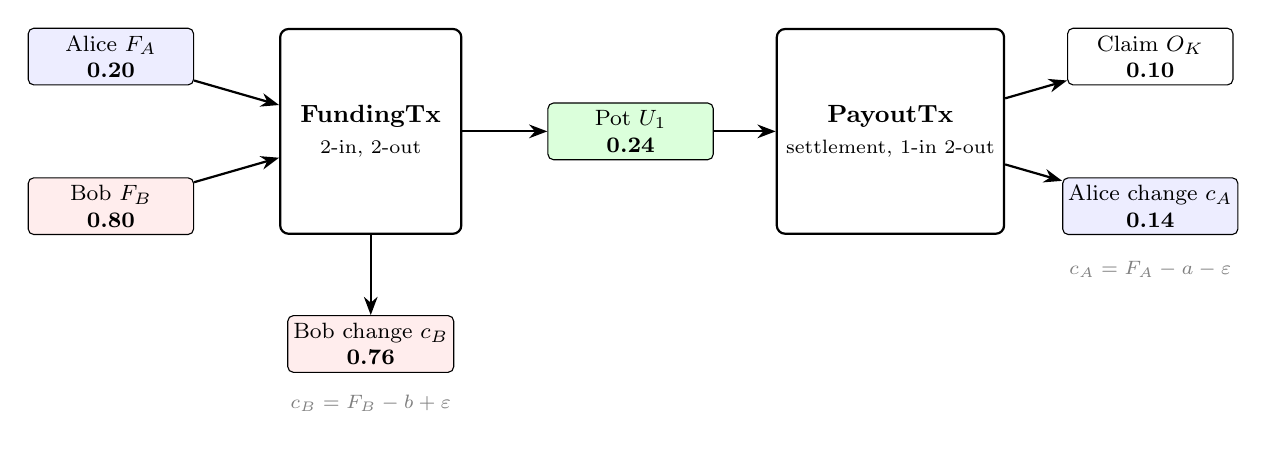
\begin{tikzpicture}[
  >=Stealth,
  tx/.style={draw, thick, rounded corners=3pt,
             minimum width=2.3cm, minimum height=2.6cm,
             align=center, font=\small},
  io/.style={draw, rounded corners=2pt,
             minimum width=2.1cm, minimum height=0.72cm,
             align=center, font=\footnotesize, inner sep=2pt},
  arr/.style={->, thick},
  alice/.style={fill=blue!7},
  bob/.style  ={fill=red!7},
  pot/.style  ={fill=green!14},
]

% ---- Funding inputs ----
\node[io, alice] (FA) at (0, 0.95) {Alice $F_A$\\\textbf{0.20}};
\node[io, bob]   (FB) at (0,-0.95) {Bob   $F_B$\\\textbf{0.80}};

% ---- FundingTx ----
\node[tx] (F) at (3.3, 0) {\textbf{FundingTx}\\\scriptsize 2-in, 2-out};

% ---- Pot: output of FundingTx == input of PayoutTx ----
\node[io, pot] (U1) at (6.6, 0) {Pot $U_1$\\\textbf{0.24}};

% ---- Bob's change (output of FundingTx) ----
\node[io, bob] (CB) at (3.3,-2.7) {Bob change $c_B$\\\textbf{0.76}};

% ---- PayoutTx (pre-signed settlement) ----
\node[tx] (P) at (9.9, 0) {\textbf{PayoutTx}\\\scriptsize settlement, 1-in 2-out};

% ---- Payout outputs ----
\node[io]        (OK) at (13.2, 0.95) {Claim $O_K$\\\textbf{0.10}};
\node[io, alice] (CA) at (13.2,-0.95) {Alice change $c_A$\\\textbf{0.14}};

% ---- arrows ----
\draw[arr] (FA) -- (F);
\draw[arr] (FB) -- (F);
\draw[arr] (F)  -- (U1);
\draw[arr] (F)  -- (CB);
\draw[arr] (U1) -- (P);
\draw[arr] (P)  -- (OK);
\draw[arr] (P)  -- (CA);

% ---- sweetener annotations ----
\node[font=\scriptsize, gray] at (3.3,-3.45) {$c_B = F_B - b + \varepsilon$};
\node[font=\scriptsize, gray] at (13.2,-1.75){$c_A = F_A - a - \varepsilon$};

\end{tikzpicture}
\caption{Pot-sweetener example (\S3.6). Equal stakes $a=b=0.05$ give an at-risk pot
$S=a+b=0.10$; Alice adds a sweetener $\varepsilon=0.01$ favouring Bob. Alice funds
$F_A=0.20$, Bob funds $F_B=0.80$. The sweetener is borne entirely by the two change
outputs~---~Bob's grows by $\varepsilon$, Alice's shrinks by $\varepsilon$~---~so the
intermediate pot becomes $U_1 = F_A + b - \varepsilon = 0.24$ while the at-risk claim
$O_K = S = 0.10$ is unchanged. In expectation Alice forgoes $\varepsilon$ and Bob gains
$\varepsilon$.}
\label{fig:sweetener}
\end{figure}

\section{Construction of the proof $\pi_A$}
\label{sec:pia}

$\pi_A$ proves the relation $\mathcal{R}_{\pi_A}$ of Definition~\ref{def:piA} for a chosen ``pad'' function $f$. We'll present a line of reasoning leading to a sensible choice for $f$.

\subsection{The broken case: $f(t)=t$}

The fact that this doesn't work is instructive. If we write $\textrm{ctxt} = a_c + t \ \textrm{mod}\ p$, it seems plausible, because the dlog $a_c$ is computationally hidden by a random field element $t$. But in fact in this case Bob can use the ciphertext to immediately derive the information on whether his guess was correct, without receiving the adaptor completion (i.e. without needing to wait until he receives the dlog $t$). The problem is that this relation is \textbf{linear}: he can compute $\textrm{ctxt}\,G - T = (a_c + t)G - tG = a_c G = A_c$, directly recovering \emph{which} thimble Alice encrypted --- hence her choice $c$ --- and comparing it against his guess $A_y$ he learns the outcome before the adaptor completes, so he can abort if he is losing.

This is a consequence of the homomorphism of the group operation. The insight that follows is, $f$ needs to be non-affine. Which leaves a substantial open question about whether it needs more structure than that. Hence the next option:

\subsection{Squaring pad: $f(t)=t^2$}
\label{sec:squaring-proof}

Take $f(t)=t^2$, so $\textrm{ctxt}=a_c+t^2$. Define the branch targets $Y_i := \textrm{ctxt}\,G - A_i$ for $i\in\{1,2\}$. On the true branch,
\[
Y_c = (\textrm{ctxt}-a_c)\,G = t^2\,G = t\,(tG) = t\,T,
\]
so the entire relation $\mathcal{R}_{\pi_A}$ collapses, for this $f$, to
\[
\exists\,c\in\{1,2\},\ t\in\mathbb{F}_p:\qquad T = t\,G\ \ \wedge\ \ Y_c = t\,T.
\]
This is a $1$-of-$2$ CDS OR \cite{cds} of Chaum--Pedersen equal-discrete-log proofs \cite{chaumpedersen}, $\mathrm{DLEQ}(G,T;\,T,Y_c)$: one witness $t$, proved to be simultaneously the discrete log of $T$ base $G$ and of $Y_c$ base $T$.

\subsubsection{Squaring proof construction}

\begin{itemize}
\item Choose $a_i \stackrel{\$}{\leftarrow} \mathbb{Z}_p$ and the adaptor secret $t \stackrel{\$}{\leftarrow} \mathbb{Z}_p$ (the $a_i$ were chosen before PayoutTx construction by Alice, but we emphasize the source of their choice here, as it is crucial to the security argument).
\item Given the choice $c$ from $1,2$ by Alice, construct $T = tG$ and the ciphertext $\textrm{ctxt} = a_c + t^2\ \textrm{mod}\ p$.
\item Construct $Y_i = \textrm{ctxt}G - A_i,\ i \in 1,2$
\item Choose commitment nonce $r_c \stackrel{\$}{\leftarrow} \mathbb{Z}_p$ (remember that $c$ is \emph{Alice's} choice from $1,2$) and note the corresponding commitment points $R_{c,T} = r_c T$, $R_{c,G} = r_c G$.
\item Deduce commitment points for the fake branch of the CDS proof, i.e. for $i \ne c$. Choose : $e_i \stackrel{\$}{\leftarrow} \mathbb{Z}_p$ and $s_i \stackrel{\$}{\leftarrow} \mathbb{Z}_p$. Then set $R_{i,T} = s_i T - e_i Y_i$ and $R_{i,G} = s_i G - e_i T$.
\item Calculate the Fiat-Shamir hash challenge: $e = H(\textrm{DOM}, A_1, A_2, T, \textrm{ctxt}, R_{..})$ where $R_{..}$ stands in for all 4 of the aforementioned commitment values. Here ``DOM'' is intended to stand in for some domain-tagging string.
\item We now apply the CDS OR-proof idea: the challenges used for the two statements under OR must add (mod p) to the FS-challenge: $e_1 + e_2 = e\ \textrm{mod}\ p$. This gives us a specific value for $e_c$.
\item Complete the sigma protocol for DLEQ on the ``honest'' branch: $s_c = r_c + e_c t\ \textrm{mod}\ p$.
\item Publish the ciphertext and proof as $\textrm{ctxt}, T, R_{..}, s_1, s_2, e_1, e_2$.
\end{itemize}

(A bandwidth optimization would be to remove the $R_{..}$ values and only publish the challenges $e$, but this is an implementation detail).

\subsubsection{Squaring proof verification}

On receipt of the tuple $\textrm{ctxt}, T, R_{..}, s_1, s_2, e_1, e_2$, Bob does the following:

\begin{itemize}
\item He first reconstructs both $Y_1$ and $Y_2$. These are $Y_i = \textrm{ctxt}G - A_i$. Notice how, unlike the broken linear case, this does \emph{not} allow him to deduce the correct choice: $Y_c = tT$ but by the DDH assumption\footnote{technically it's the square DDH assumption, because it's one exponent $t$ repeated, not two}, Bob cannot distinguish between the correct and wrong choice.
\item He reconstructs the Fiat-Shamir challenge: $e = H(\textrm{DOM}, A_1, A_2, T, \textrm{ctxt}, R_{..})$
\item He verifies on the $T$-branch: $s_i T \stackrel{?}{=} R_{i,T} + e_i Y_i,\ i \in 1,2$
\item He verifies on the $G$-branch: $s_i G \stackrel{?}{=} R_{i,G} + e_i T,\ i \in 1,2$
\item He verifies $e = e_1 + e_2\ \mod\ p$
\end{itemize}

\subsubsection{Squaring proof security: hiding}
Security of the branch-hiding rests on a square-DDH assumption (distinguishing $(G,tG,t^2G)$ from $(G, tG, \textrm{random}G)$). One caveat is intrinsic to squaring: the mask $t^2$ ranges over quadratic residues, so for a \emph{guessable} candidate $a$ the value $\textrm{ctxt}-a$ can be tested for quadratic residuosity, passing always for the true $a$ and with probability $\approx\tfrac12$ for a random false one. The hiding property is therefore sound only for \emph{high-entropy} masked scalars --- which the thimble scalars $a_1,a_2$ and $t$ are, being sampled uniformly from $\mathbb{F}_p$. It must not be used to hide low-entropy plaintexts (amounts, counters, votes). See Appendix A for the detailed reduction proof.

Note that the proof would be totally unsound in a DDH-easy group (because DDH easy $\Rightarrow$ square-DDH easy); but secp256k1 is a DDH-hard group, because it is prime order and has no efficiently-computable pairing.

An additional point is that square-DDH is \emph{not} reducible to DDH, or at least no such reduction is known.

\subsubsection{Squaring proof security: soundness}
% Requires: \usepackage{amsthm,amssymb}
The soundness of the proof is relatively simple; it's 2-special soundness in the ROM of the relevant hash function:

\begin{lemma}[Knowledge soundness of $\pi_A$]
  The squaring-pad proof $\pi_A$ of Section~\ref{sec:squaring-proof} is a
  proof of knowledge for the relation
  $$
    \mathcal R_{\pi_A}
    =
    \left\{
      (\mathsf{ctxt},T,A_1,A_2);\,
      (t,c,a_c):
      c\in\{1,2\},\,
      T=tG,\,
      A_c=a_cG,\,
      \mathsf{ctxt}=a_c+t^2 \bmod p
    \right\}.
  $$
\end{lemma}

\begin{proof}[Sketch]
  Recall that $\pi_A$ is a 1-of-2 CDS-OR of Chaum--Pedersen proofs of
  equal discrete logarithms:
  $$
    \operatorname{DLEQ}(G,T;\,T,Y_i),
    \qquad
    Y_i = \mathsf{ctxt}\cdot G - A_i,
    \qquad i\in\{1,2\}.
  $$
  Each branch is a standard proof of knowledge of $t$ satisfying
  $tG=T$ and $tT=Y_i$, and therefore has 2-special soundness: from two
  accepting transcripts with the same commitments but different
  challenges, an extractor recovers
  $$
    t = \frac{s_i - s'_i}{e_i - e'_i} \bmod p.
  $$

  The CDS-OR composition preserves this property. Given two accepting
  transcripts with distinct total challenges $e\neq e'$, where
  $e=e_1+e_2$ and $e'=e'_1+e'_2$, at least one branch has
  $e_i\neq e'_i$. Special soundness on that branch extracts $t$ (note that this is true independent of which branch is extracted; the corresponding secret in both cases is $t$).

  Once $t$ is known, the ciphertext determines the encrypted thimble
  scalar:
  $$
    a_c = \mathsf{ctxt} - t^2 \bmod p.
  $$
  Checking which published thimble satisfies $a_c G = A_c$ identifies
  the branch $c$ and completes the witness.
\end{proof}

\subsection{ZK-friendly hash pad: $f=\mathrm{Poseidon}$}

This is speculative, and would need the input of experts, though at a high level, it is very clearly possible.

Taking $f$ to be a hash makes $\textrm{ctxt}=a_c+f(t)$ a non-affine relation. We prove it in zero knowledge with a transparent Bulletproofs \cite{bulletproofs} R1CS instantiated over secp256k1 (using the Curve Trees generic-curve backend \cite{curvetrees}), where $f$ is a Poseidon \cite{poseidon} permutation over $\mathbb{F}_p$ --- field-native, with the $x^5$ S-box (valid since $\gcd(5,p-1)=1$) --- together with a sigma conjunct binding $a_c$ to a published thimble and $t$ to $T$. This gives a general (any hash-like $f$) route at higher cost: a few hundred multiplication gates, i.e.\ order $10^2$~ms to prove and a $\sim\!1$~KB proof, still with no trusted setup. A reviewed, field-native alternative to a hand-parameterised Poseidon is the Purify PRF of MuSig-DN \cite{musigdn}, an algebraic PRF whose output already lands in the circuit's scalar field.

\underline{In summary:}

The squaring construction is complete and cheap but couples $f$ to $t^2$; the hash construction admits an arbitrary $f$ at a cost. Which is preferable --- and whether reference parameters or a reviewed PRF should replace the hand-rolled Poseidon --- is left to future work.


\section{Cooperative Alice-payout completion}
\label{sec:coop}

The enforced payout path of the simplest description of Section~\ref{sec:crypto} leaves exactly one non-payment-like footprint: when Bob loses, Alice reclaims $O_K$ through the CSV script leaf, revealing a tapscript rather than spending by a key path. We have avoided this problem in our detailed protocol description -- in this section we'll describe the reasoning behind the CooperativeOverlayTx that enables this.

Once the outcome is determined, rather than broadcasting the PayoutTx, Alice sends $t$ to Bob off-chain. Bob checks $tG=T$, computes $a_c=\textrm{ctxt}-f(t)$, and --- finding $a_c G\neq A_y$, i.e.\ that he lost ($y\neq c$) --- co-signs with Alice a plain MuSig2 key-path spend of the pot $U_1$ directly to a fresh destination of Alice's. No PayoutTx ever reaches the chain: the new payout (``Cooperative Overlay'') is an ordinary taproot key-path payment, indistinguishable from a normal transfer.

Bob has no incentive to refuse: he has lost regardless, so withholding his signature only delays Alice, and the enforced settlement-then-CSV path remains available as a backstop if he stalls. Thus in the common (honest) case \emph{both} outcomes --- Bob-wins (already a key-path spend of $O_K$) and Alice-wins (this cooperative key-path spend of $U_1$) --- are plain payments. The aggregated construction of \S\ref{sec:agg} generalizes exactly this cooperative overlay from a single bet to a batch of them.


\section{Aggregated bets: de-quantizing the payout}
\label{sec:agg}

The single bet of \S\ref{sec:crypto}, even in its $1$-of-$N$ form, leaves one residual fingerprint that the payment-shaping of \S\ref{sec:pst} does \emph{not} remove: the payout \emph{amount}. An even-money bet pays $0$ or $2a$; a $1$-of-$N$ bet pays $0$ or $Ns$. Either way the claim output takes one of a small number of values on a grid fixed by the stake --- and that grid is partly recoverable by an observer, because the funding transaction reveals the pot size. A settlement output equal to exactly twice a plausible stake is a weak but real tell that a \emph{bet}, rather than an arbitrary payment, occurred.

This section describes an overlay --- implemented in the reference code \cite{babilonia} --- that removes this tell while keeping the two-transaction covert footprint intact. It introduces \textbf{no new cryptographic assumption}: it composes $k$ independent instances of the single-bet primitive of \S\ref{sec:crypto} and merges their outcomes with a cooperative novation that is exactly the \S\ref{sec:coop} overlay, generalized from one bet to $k$.

\subsection{Construction}

Fix a session parameter $k$ (the reference implementation uses $k=5$). The player's total stake $S_B$ is split, \emph{at random and in unequal, un-quantized amounts}, across $k$ sub-bets,
\[
S_B \ =\ \sum_{i=1}^{k} s_i ,
\]
where sub-bet $i$ is an independent $1$-of-$N_i$ game (\S\ref{sec:nary}) with its own thimbles, its own player stake $s_i$, and its own hidden guess. Each sub-bet carries its own $\pi_A,\pi_B$; the fairness of sub-bet $i$ depends on no other sub-bet.

All $k$ sub-bets are funded into a \emph{single} pot $U_1$, exactly as in \S\ref{sec:pst}. For a fair $1$-of-$N_i$ game the dealer fronts $(N_i-1)s_i$, so sub-bet $i$'s at-risk amount is $S_i = N_i s_i$, and the pot must cover the worst case in which the player wins every sub-bet:
\[
U_1 \ \ge\ \sum_{i=1}^{k} N_i s_i \ +\ \text{fees},
\qquad\text{with dealer front} \ =\ \sum_{i=1}^{k}(N_i-1)\,s_i .
\]
This solvency bound is checked before the player signs funding, so an under-capitalised dealer is rejected up front rather than mid-protocol. When the outcomes are determined, the player's gross receipt is the subset-sum of the sub-bets he won,
\[
\mathrm{net}_B \ =\ \sum_{i \,:\, y_i = c_i} N_i s_i ,
\]
his net profit-and-loss being $\mathrm{net}_B - S_B$; the remainder $U_1 - \mathrm{net}_B - \text{fee}$ returns to the dealer (her stake, her front on the sub-bets the player lost, and her change).

\subsection{Cooperative novation into one settlement}

Settling $k$ sub-bets as $k$ separate on-chain events would destroy both the covert footprint and the cost advantage. Instead the parties pre-sign an \emph{enforcement graph} --- a splitter transaction spending $U_1$ into $k$ sub-pots, each with its own settlement/refund exactly as in \S\ref{sec:crypto} --- but treat it purely as a fallback. On the happy path they \textbf{cooperatively novate}: once every sub-bet's outcome is known to both parties, they agree the single net figure $\mathrm{net}_B$ and co-sign one key-path spend of $U_1$, the \emph{Aggregate settlement}, paying $\mathrm{net}_B$ to the player and the balance to the dealer. This is a single ordinary two-output payment (Figure~\ref{fig:agg}).

The incentive argument is the one from \S\ref{sec:coop}, extended: the aggregate and the enforcement graph are alternative valid spends of the same pot that resolve to the \emph{identical} net for both parties, so broadcasting the graph is strictly dominated --- it costs more in fees and gains nothing. Cooperation is therefore self-enforcing, and the (rarely used) enforcement graph guarantees that neither party can be cheated by the other's refusal to novate.

\begin{figure}[h]
\centering
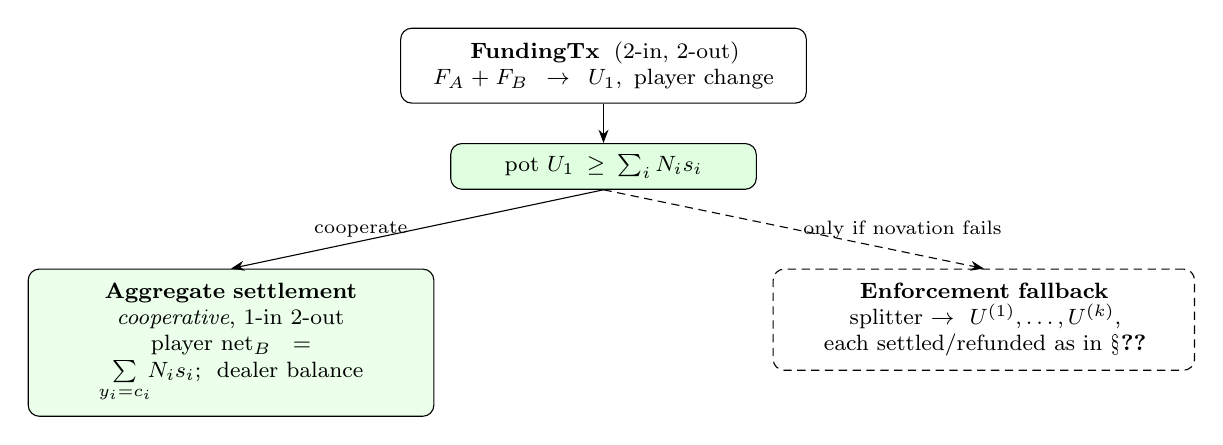
\begin{tikzpicture}[>=Stealth,
  tx/.style={draw, rounded corners, align=center, inner sep=5pt, font=\footnotesize, text width=4.8cm},
  pot/.style={draw, rounded corners, align=center, inner sep=4pt, font=\footnotesize, fill=green!12, text width=3.6cm},
  fb/.style={draw, densely dashed, rounded corners, align=center, inner sep=5pt, font=\footnotesize, text width=5.0cm},
  ann/.style={font=\scriptsize}]
\node[tx] (fund) {\textbf{FundingTx} \;(2-in, 2-out)\\ $F_A + F_B \;\to\; U_1,\ \text{player change}$};
\node[pot, below=5mm of fund] (u1) {pot $U_1 \ge \sum_i N_i s_i$};
\node[tx, fill=green!8, below left=10mm and 2mm of u1] (agg) {\textbf{Aggregate settlement}\\ \emph{cooperative}, 1-in 2-out\\ player $\mathrm{net}_B = \!\!\sum\limits_{y_i=c_i}\!\! N_i s_i$;\ \ dealer balance};
\node[fb, below right=10mm and 2mm of u1] (split) {\textbf{Enforcement fallback}\\ splitter $\to U^{(1)},\dots,U^{(k)}$,\\ each settled/refunded as in \S\ref{sec:crypto}};
\draw[->] (fund) -- (u1);
\draw[->] (u1.south) -- (agg.north) node[midway, left, ann] {cooperate};
\draw[->, densely dashed] (u1.south) -- (split.north) node[midway, right, ann] {only if novation fails};
\end{tikzpicture}
\caption{\textbf{Aggregated bet.} $k$ sub-bets fund one pot $U_1$; on the happy path the parties co-sign a single \emph{Aggregate settlement} paying the player his net across all $k$ (a plain two-output payment), and the pre-signed per-sub-bet enforcement graph is used only as a fallback. Both spends of $U_1$ resolve to the identical net, so cooperation is self-enforcing.}
\label{fig:agg}
\end{figure}

\subsection{Why this de-quantizes the amount}

The single bet's payout lives on a coarse grid --- $\{0, Ns\}$ for a $1$-of-$N$ bet --- and the pot size (hence $s$, hence the grid spacing) leaks from the funding transaction. The aggregate payout, by contrast, is a subset-sum
\[
\mathrm{net}_B \ =\ \sum_{i \,:\, y_i=c_i} N_i s_i
\]
of $k$ terms whose stakes $s_i$ are \emph{independently random and un-quantized} (the implementation samples them coprime, at $1$-sat resolution). The set of achievable payouts is therefore dense and carries no fixed even-money spacing: the settlement output reads as an arbitrary amount, not as $2\times$ a round stake. By the central limit theorem the aggregate net concentrates around $S_B$ with a spread of order $S_B/\sqrt{k}$ and \emph{no} atom at a ``doubled-stake'' value --- the recognizable $\times 2$ comb of the even-money bet is gone. This is the crux of the construction: it is the odds diversity and the un-quantized split, \emph{not} a large $N$, that buy amount-covertness, and they do so while the on-chain footprint remains exactly the two-transaction payment shape of \S\ref{sec:pst}.

Every recovery path of \S\ref{sec:crypto} survives unchanged. If novation fails, the enforcement graph settles each sub-bet independently (splitter, then per-sub-bet settlement/claim or timeout refund), and the pre-signed refund of the whole pot remains the player's principal-safe backstop before funding is ever broadcast.


\section{Network communication layer}
\label{sec:netlayer}

Two network-layer needs remain: an off-chain channel over which the two parties negotiate the protocol, and a way to \emph{discover} counterparties in the first place. Both can be met by mechanisms that are themselves covert --- so that not even the existence of a negotiation is visible to third parties --- pairing naturally with the payment-shaped on-chain footprint of Section~\ref{sec:pst}.

\subsection{BIP324 decoy packets}

If BIP324 \cite{bip324} P2P encryption is used --- as it now is for the majority of global Bitcoin P2P traffic, having been enabled by default since Bitcoin Core~27.0 \cite{optechv2} --- then it is possible for individual nodes to send decoy packets that are not distinguishable from the true P2P traffic. This is one way for first-class Bitcoin users (that is, users who actually fully verify payments with their own node) to negotiate the Babilonia protocol to bet with each other trustlessly, and in theory, without anyone else knowing they're doing it.

It's exactly in this use-case scenario where it would be especially advantageous to have the onchain trace of the betting protocol look purely like payments.

To support this at the network layer, a very simple patch to Bitcoin Core may be enough.\footnote{A proof-of-concept patch adding \texttt{senddecoy}/\texttt{getdecoys} RPCs is included with the reference implementation \cite{babilonia}.} Having said this, it's obvious that this is far from the only way to exchange messages privately! It's just one that's quite serendipitous: it aligns with privacy and security conscious bitcoin usage, and even provides a slight incentive to run more Bitcoin nodes, which is healthy for the network.

\subsection{Discovery and Sybil attacks}

Both in the case of communicating full nodes or Babilonia users communicating otherwise, there is the natural problem of how to discover counterparties. We leave a concrete rendezvous mechanism to future work.

As an extreme, consider that sending BIP324 decoy requests, that are ignored by vanilla Core nodes, but considered and potentially accepted by Babilonia-patched nodes, allows anonymous parties to engage in this protocol. The fact that this is even possible is of course a direct result of the fully trustless fair bet protocol created by the cryptography.

Naive implementation is, like any other anonymous protocol, open to Sybil attacks. This can be addressed with cost imposition (amongst other more brittle solutions) - a huge topic that we won't address here.


\section{Example implementation}

See \url{https://github.com/AdamISZ/babilonia}. The code is largely written by Claude Opus 4.8 as of now, and therefore carries a ``do not use with real money'' warning, though it would need review in any case. However, it has been tested on signet as being functional. To use, patch 2 or more Bitcoin Core nodes with the provided patch (or simply test locally on regtest).

The reference implementation covers both the single bet (node-to-node over the BIP324 covert channel of \S\ref{sec:netlayer}) and the aggregated construction of \S\ref{sec:agg}: it uses $k=5$ sub-bets, each a $1$-of-$N$ game with $N$ drawn from $\{2,\dots,5\}$, and merges them by cooperative novation into a single settlement. It also ships a browser player client --- a WebAssembly build of the same protocol crate --- in which the player's own external wallet co-signs the funding PSBT, so the player custodies their coins throughout.

As of the time of writing, this implementation has no ``pot-sweetener'' function, but it is not hard to add.

\section{Other similar ideas}
\label{sec:ideas}

If we take the core idea here as ``not-balance-preserving but cryptographically fair collaborative transactions'' and, as noted, this can have some significant benefits in terms of obscuring transaction history, there are a few different other directions one could look at it, than this very simple ``probabilistic coinjoin with covert properties''. For example:

\begin{itemize}
\item The same but applied to 2 party privacy perserving coinswaps \cite{coinswap}: their main disadvantage is their equal-amount fingerprint, which had previously been addressed with splitting. This construction, or that of GTT \cite{gerhardt2026}, could address this.
\item A not-covert (i.e. no steganographic) large scale coinjoin a la Wasabi or similar, but with an inbuilt lottery. This could incentivize (possibly?) usage of larger user groups. Achieving that outcome trustlessly seems non-trivial
\item Just a lottery generally, in one of these or another form
\item Probabilistic swaps may have several other applications as was briefly reviewed in \cite{gerhardt2026}
\end{itemize}

\ldots and perhaps many others I haven't thought of.

\section{Acknowledgements}

Thanks to O. Kurbatov (author of \cite{kurbatov2025oprand}) for a correction to (\S3.3) as the protocol messaging order was the more inefficient version; this corrected version (which matches the implementation in \ref{sec:ideas}) prevents the players having to wait for funding confirmation in order to do bet setup, which makes it far more practical (that is, it makes a fallback to a refund transaction far less likely).

\begin{thebibliography}{99}

\bibitem{chaum1981} D.~Chaum. Untraceable electronic mail, return addresses, and digital pseudonyms. \emph{Communications of the ACM}, 24(2):84--90, 1981.

\bibitem{maxwell2013} G.~Maxwell. CoinJoin: Bitcoin privacy for the real world. BitcoinTalk, 2013. \url{https://bitcointalk.org/index.php?topic=279249.0}

\bibitem{zerolink} \'A.~Ficsor et al. ZeroLink: The Bitcoin fungibility framework, 2017. (Basis of the Wasabi and Samourai/Whirlpool equal-output CoinJoins.)

\bibitem{wabisabi} \'A.~Ficsor, L.~Hangyi, K.~Kravchenko, G.~Kajd\'i, Y.~Sun, T.~Bab\'o. WabiSabi: Centrally coordinated CoinJoins with variable amounts. IACR ePrint 2021/206. \url{https://eprint.iacr.org/2021/206}

\bibitem{lightning} J.~Poon and T.~Dryja. The Bitcoin Lightning Network: Scalable off-chain instant payments, 2016. \url{https://lightning.network/lightning-network-paper.pdf}

\bibitem{payjoin} N.~Dorier. BIP~78: A simple Payjoin proposal, 2019. \url{https://github.com/bitcoin/bips/blob/master/bip-0078.mediawiki}

\bibitem{satoshidice} Satoshi Dice. Bitcoin Wiki. \url{https://en.bitcoin.it/wiki/Satoshi_Dice}

\bibitem{kurbatov2025oprand} O.~Kurbatov. Emulating OP\_RAND in Bitcoin. arXiv:2501.16451, 2025. \url{https://arxiv.org/abs/2501.16451}

\bibitem{gerhardt2026} P.~Gerhart, J.~Taylor, S.~A.~K.~Thyagarajan. Probabilistic Atomic Swaps for Bitcoin and Friends. arXiv:2605.04975, 2026. \url{https://arxiv.org/abs/2605.04975}

\bibitem{musig2} J.~Nick, T.~Ruffing, Y.~Seurin. MuSig2: Simple two-round Schnorr multi-signatures. \emph{CRYPTO 2021}; IACR ePrint 2020/1261. \url{https://eprint.iacr.org/2020/1261}

\bibitem{bip327} J.~Nick, T.~Ruffing, Y.~Seurin. BIP~327: MuSig2 for BIP340-compatible multi-signatures, 2022. \url{https://github.com/bitcoin/bips/blob/master/bip-0327.mediawiki}

\bibitem{fournier} L.~Fournier. One-time verifiably encrypted signatures, a.k.a. adaptor signatures, 2019. \url{https://github.com/LLFourn/one-time-VES/blob/master/main.pdf}

\bibitem{cds} R.~Cramer, I.~Damg\aa rd, B.~Schoenmakers. Proofs of partial knowledge and simplified design of witness hiding protocols. \emph{CRYPTO 1994}, LNCS 839, 174--187.

\bibitem{chaumpedersen} D.~Chaum, T.~P.~Pedersen. Wallet databases with observers. \emph{CRYPTO 1992}, LNCS 740, 89--105.

\bibitem{bulletproofs} B.~B\"unz, J.~Bootle, D.~Boneh, A.~Poelstra, P.~Wuille, G.~Maxwell. Bulletproofs: Short proofs for confidential transactions and more. \emph{IEEE S\&P 2018}. \url{https://eprint.iacr.org/2017/1066}

\bibitem{curvetrees} M.~Campanelli, M.~Hall-Andersen, S.~E.~Kamp. Curve Trees: Practical and transparent zero-knowledge accumulators. \emph{USENIX Security 2023}. \url{https://eprint.iacr.org/2022/756}

\bibitem{poseidon} L.~Grassi, D.~Khovratovich, C.~Rechberger, A.~Roy, M.~Schofnegger. Poseidon: A new hash function for zero-knowledge proof systems. \emph{USENIX Security 2021}. \url{https://eprint.iacr.org/2019/458}

\bibitem{musigdn} J.~Nick, T.~Ruffing, Y.~Seurin, P.~Wuille. MuSig-DN: Schnorr multi-signatures with verifiably deterministic nonces. \emph{ACM CCS 2020}; IACR ePrint 2020/1057. \url{https://eprint.iacr.org/2020/1057}

\bibitem{fistful} S.~Meiklejohn, M.~Pomarole, G.~Jordan, K.~Levchenko, D.~McCoy, G.~M.~Voelker, S.~Savage. A fistful of Bitcoins: characterizing payments among men with no names. \emph{ACM IMC 2013}. \url{https://cseweb.ucsd.edu/~smeiklejohn/files/imc13.pdf}

\bibitem{bip341} P.~Wuille, J.~Nick, A.~Towns. BIP~341: Taproot: SegWit version 1 spending rules, 2020. \url{https://github.com/bitcoin/bips/blob/master/bip-0341.mediawiki}

\bibitem{oprf} A.~Davidson, A.~Faz-Hern\'andez, N.~Sullivan, C.~A.~Wood. RFC~9497: Oblivious Pseudorandom Functions (OPRFs) using prime-order groups, 2023. \url{https://www.rfc-editor.org/rfc/rfc9497}

\bibitem{bip324} P.~Wuille, D.~Mehta, T.~Ruffing, J.~Schnelli. BIP~324: Version~2 P2P encrypted transport protocol. \url{https://github.com/bitcoin/bips/blob/master/bip-0324.mediawiki}

\bibitem{optechv2} Bitcoin Optech. Version~2 P2P transport. \url{https://bitcoinops.org/en/topics/v2-p2p-transport/}

\bibitem{antifeesniping} Bitcoin Optech. Fee sniping. \url{https://bitcoinops.org/en/topics/fee-sniping/}

\bibitem{babilonia} Babilonia reference implementation. \url{https://github.com/AdamISZ/babilonia}

\bibitem{coinswap} Citadel Tech. Coinswap: a trustless, peer-to-peer implementation of the Maxwell--Belcher CoinSwap protocol. \url{https://github.com/citadel-tech/coinswap}

\bibitem{kelly} J.~L.~Kelly~Jr. A new interpretation of information rate. \emph{Bell System Technical Journal}, 35(4):917--926, 1956.

\bibitem{payjoinblog} waxwing. Payjoin blog post Jan 2019 \url{https://web.archive.org/web/20201108034458/https://joinmarket.me/blog/blog/payjoin/}

\bibitem{joinmarket} Joinmarket, original author Chris Belcher. See \url{https://en.bitcoin.it/wiki/JoinMarket}

\end{thebibliography}

\newpage

\section{Appendix A: Reduction of the squaring proof to square-DDH}

We assume the existence of an adversary $\mathcal{A}^{WFP}$ who with non-negligible probability can, given the output the protocol of section 4.2.1-4.2.3: $\textrm{ctxt}, T, \sigma'_{A, P}$ with the pre-determined thimbles $A_1, A_2$, whether the choice was $c=1$ or $c=2$.

We show that this adversary solves the square-DDH problem with non-negligible probability.

\paragraph{Square Decisional Diffie--Hellman (sqDDH).}
Let $G$ be a group of prime order $p$ with generator $G$, written
additively. The \emph{square-DDH} advantage of an adversary $\mathcal{A}$
is defined as
$$
\operatorname{Adv}^{\mathrm{sqDDH}}_{\mathcal{A}}(p)
=
\left|
\Pr\!\big[\mathcal{A}(G,\, tG,\, t^{2}G)=1 \;\big|\; t \xleftarrow{\$} \mathbb{Z}_{p}\big]
-
\Pr\!\big[\mathcal{A}(G,\, tG,\, uG)=1 \;\big|\; t,u \xleftarrow{\$} \mathbb{Z}_{p}\big]
\right|.
$$
The \emph{square-DDH assumption} holds in $G$ if for every probabilistic
polynomial-time adversary $\mathcal{A}$, this advantage is negligible in
$\log p$.

Game Square-DDH:

\paragraph{Game $\mathsf{sqDDH}_{\mathcal{G}, \mathcal{A}}(\lambda)$.}
Let $\mathcal{G} = (G, p, G)$ be a description of a cyclic group of prime
order $q$ generated by $G$, sampled by
$\mathsf{GroupGen}(1^{\lambda})$, where $\lambda$ is the security
parameter. The game proceeds between a challenger $\mathcal{C}$ and an
adversary $\mathcal{A}$ as follows:

\begin{enumerate}
  \item \textbf{Setup.} The challenger runs
    $\mathcal{G} \gets \mathsf{GroupGen}(1^{\lambda})$, obtaining
    $(G, p, G)$, and samples
    $t \xleftarrow{\$} \mathbb{Z}_{p}$.

  \item \textbf{Challenge.} The challenger samples a bit
    $b \xleftarrow{\$} \{0, 1\}$.
    \begin{itemize}
      \item If $b = 0$ (\emph{real}), set $Y \gets t^{2}G$.
      \item If $b = 1$ (\emph{random}), sample
        $u \xleftarrow{\$} \mathbb{Z}_{p}$ and set $Y \gets uG$.
    \end{itemize}
    The challenger sends the tuple $(G, p, G,\; T,\; Y)$, where
    $T \gets tG$, to the adversary $\mathcal{A}$.

  \item \textbf{Guess.} $\mathcal{A}$ outputs a bit
    $b' \in \{0, 1\}$.
\end{enumerate}

\medskip\noindent
\textbf{Winning condition.} $\mathcal{A}$ wins the game if $b' = b$.
We define the advantage of $\mathcal{A}$ in the square-DDH game as
$$
\operatorname{Adv}^{\mathsf{sqDDH}}_{\mathcal{G},\mathcal{A}}(\lambda)
\;=\;
\left|
  \Pr\!\big[\mathsf{sqDDH}_{\mathcal{G},\mathcal{A}}(\lambda) = 1\big]
  \;-\;
  \frac{1}{2}
\right|.
$$
The \emph{square-DDH assumption} holds with respect to
$\mathsf{GroupGen}$ if for every probabilistic polynomial-time adversary
$\mathcal{A}$,
$\operatorname{Adv}^{\mathsf{sqDDH}}_{\mathcal{G},\mathcal{A}}(\lambda)$
is negligible in $\lambda$.

We define the entity $C^{sqddh}$ as the challenger for Game sqDDH. We define the entity $R$ as the adversary for Game sqDDH and as challenger for Game WFP. And we define $\mathcal{A}^{WFP}$, as noted, as the adversary assumed to be able to win Game WFP. As shown in Table~\ref{tab:sqddh-reduction} $R$ can use $\mathcal{A}^{WFP}$ to win Game sqDDH by programming the RO for $\mathcal{A}^{WFP}$. Note that $R$ must choose $a_1$, $a_2$ and $\textrm{ctxt}$ randomly from $\mathbb{Z}_p$ so that the inputs to $\mathcal{A}^{WFP}$ are indistinguishable from a normal run of Game WFP. It's for this reason that the proof does \emph{not} hold if any of the quantities $a_1, a_2, t$ are not chosen purely at random from $\mathbb{Z}_p$ (for example, if they are chosen from an enumerable set).

\begin{table}[h]
\centering
\footnotesize
\renewcommand{\arraystretch}{1.45}
\begin{tabular}{|c|p{3.4cm}|p{6.3cm}|p{3.0cm}|}
% manual rebalance — make "Sends" wider, "Does" much wider,
% and drop the unused "Step" column or shrink it:
\hline
\textbf{Step} & \textbf{$C^{\mathrm{sqddh}}$ (sqDDH challenger)} & \textbf{$R$ (sqDDH adversary \& WFP challenger)} & \textbf{$\mathcal{A}^{\mathrm{WFP}}$ (WFP adversary)} \\
\hline
1 &
Samples $t\xleftarrow{\$}\mathbb{Z}_p$,\; $b\xleftarrow{\$}\{0,1\}$.
If $b{=}0$: $Y\leftarrow t^{2}G$.
If $b{=}1$: $u\xleftarrow{\$}\mathbb{Z}_p$,\; $Y\leftarrow uG$.
Sets $T\leftarrow tG$.
Sends $(G,\,T,\,Y)$. & & \\
\hline
2 & &
Receives $(G,\,T,\,Y)$.
Guesses $c\xleftarrow{\$}\{1,2\}$;\; let $j=3{-}c$ (the complement). & \\
\hline
3 & &
Samples $\textrm{ctxt}\xleftarrow{\$}\mathbb{Z}_p$ and $a_{j}\xleftarrow{\$}\mathbb{Z}_p$.
Sets $A_{j}\leftarrow a_{j}G$ and
$A_{c}\leftarrow \textrm{ctxt}\cdot G - Y$,
so that $Y_{c}=\textrm{ctxt}\cdot G - A_{c}=Y$ by construction.
 & \\
\hline
4 & &
Simulates Schnorr PoKs for $A_{1},A_{2}$:
honest for $A_{j}$ (knows $a_{j}$);
for $A_{c}$, programs the RO and simulates
(does not know $a_{c}$). & \\
\hline
5 & &
Simulates the adaptor signature $\sigma'_{A,P}$:
samples $s'\xleftarrow{\$}\mathbb{Z}_p$ and $e_{\mathrm{sig}}\xleftarrow{\$}\mathbb{Z}_p$;
sets $R_{A}\leftarrow s'G + T - e_{\mathrm{sig}}\,\mu_{A}P_{A}$;
programs $H_{\mathrm{sig}}(R_{agg},\,P_{\mathrm{agg}},\,m_{\mathrm{payout}})\leftarrow e_{\mathrm{sig}}$. & \\
\hline
6 & &
Simulates the CDS OR proof (both branches).
For each $i\in\{1,2\}$: samples $e_{i},s_{i}\xleftarrow{\$}\mathbb{Z}_p$;
computes $Y_{i}=\textrm{ctxt}\cdot G - A_{i}$;
sets $R_{i,T}\leftarrow s_{i}T - e_{i}Y_{i}$ and
$R_{i,G}\leftarrow s_{i}G - e_{i}T$.
Sets $e\leftarrow e_{1}+e_{2}\bmod p$.
Programs $H_{\mathrm{zk}}(\textrm{DOM},A_{1},A_{2},T,\textrm{ctxt},R_{\cdot\cdot})\leftarrow e$. & \\
\hline
7 & &
Sends the full transcript $\transcript$ to $\mathcal{A}^{\mathrm{WFP}}$. &
Receives the transcript;
reconstructs $Y_{1},Y_{2}=\textrm{ctxt}\cdot G-A_{i}$;
verifies the adaptor-signature equation
$s'G\stackrel{?}{=}R_{A}-T+e_{\mathrm{sig}}\mu_{A}P_{A}$
and the CDS OR equations
$s_{i}G\stackrel{?}{=}R_{i,G}+e_{i}T$,
$s_{i}T\stackrel{?}{=}R_{i,T}+e_{i}Y_{i}$,
$e_{1}+e_{2}\stackrel{?}{=}e$. \\
\hline
8 & & &
Outputs guess $c'\in\{1,2\}$. \\
\hline
9 & &
If $c'=c$: outputs $b'\leftarrow 0$ (``real / sqDDH tuple'').
If $c'\neq c$: outputs $b'\leftarrow 1$ (``random''). & \\
\hline
10 &
$R$ wins iff $b'=b$. & & \\
\hline
\end{tabular}
\caption{Reduction from WFP branch-distinguishing to sqDDH.
$R$ embeds the sqDDH challenge point $Y$ as $Y_{c}$ (the true-branch target)
and simulates the remaining transcript entirely by RO programming.
$R$ never learns $t$ or $a_{c}$.}
\label{tab:sqddh-reduction}
\end{table}

\subsection{Remarks}

\begin{itemize}
\item The only values in the transcript that can leak $c$ are the implicit $Y_1$ and $Y_2$ where $Y_i = \textrm{ctxt}G - A_i$. In the real case, exactly one of them is a sqDDH tuple $(G, T, Y_i)$, while the other is random. Distinguishing which is the sqDDH tuple is the sqDDH problem. All other transcript components (PoKs, adaptor signature, CDS OR proof) are either independent of $c$ or perfectly simulated under the traditional (RO + HVZK) model.

\item ROM requirement. The reduction programs two random oracles $\mathbb{H}_{zk}, \mathbb{H}_{sig}$ (for the CDS OR proof and the Schnorr PoKs) and (for the adaptor signature challenge) respectively. This is standard for Fiat–Shamir-based proofs.

\item The false branch $Y_j$ is always random. In both cases, $Y_j = ctxt G - a_j G$ where $a_j$ is uniform and independent (guaranteed by the random choice of ctxt), so $Y_j$ is a uniformly random element of the group, independent of $b$. This ensures that in the real case, only $Y_c$ carries the sqDDH structure, and in the random case, neither does.
\end{itemize}

\subsection{Tightness reduction}

\begin{theorem}[Tightness of the squaring-proof reduction]
\label{thm:sqddh-reduction}
Let $\mathcal{A}^{\mathrm{WFP}}$ be an adversary that, given a honestly
generated transcript
$(A_{1},A_{2},\mathrm{PoKs},\textrm{ctxt},T,\sigma'_{A,P},R_{\cdot\cdot},s_{1},s_{2},e_{1},e_{2})$
of the squaring proof from \autoref{sec:squaring-proof},
distinguishes the true branch $c\in\{1,2\}$ with advantage
$$
  \varepsilon
  \;=\;
  \Pr[c'=c]-\tfrac{1}{2},
$$
where $a_{1},a_{2},t\xleftarrow{\$}\mathbb{Z}_{p}$ are sampled uniformly
and independently. Then there exists a square-DDH adversary $R$,
running in time comparable to that of $\mathcal{A}^{\mathrm{WFP}}$ plus
the cost of simulating one transcript (a constant number of group
operations and random-oracle queries), such that
$$
  \operatorname{Adv}^{\mathrm{sqDDH}}_{R}(\lambda)
  \;\geq\;
  \tfrac{1}{2}\,\varepsilon.
$$
\end{theorem}

\begin{proof}[Sketch]
$R$ embeds the sqDDH challenge point $Y$ as $Y_{c}=\textrm{ctxt}\cdot G-A_{c}$
for a uniformly guessed $c\xleftarrow{\$}\{1,2\}$, samples
$\textrm{ctxt},a_{j}\xleftarrow{\$}\mathbb{Z}_{p}$ (with $j=3-c$),
sets $A_{c}=\textrm{ctxt}\cdot G-Y$ and $A_{j}=a_{j}G$,
and simulates the Schnorr PoKs, the adaptor signature, and the
CDS OR proof entirely by random-oracle programming; see
\autoref{tab:sqddh-reduction}.

\emph{Real case} ($b=0$, $Y=t^{2}G=tT$): then
$a_{c}=\textrm{ctxt}-t^{2}$ is uniform because $\textrm{ctxt}$ is,
and $Y_{c}=tT$ satisfies the DLEQ relation, so the simulated transcript
is distributed identically to a real one with branch $c$. Hence
$\Pr[b'=0\mid b=0]=\Pr[c'=c\mid b=0]\geq\tfrac{1}{2}+\varepsilon$.

\emph{Random case} ($b=1$, $Y=uG$): both $Y_{1},Y_{2}$ are uniform
and independent of $T$, the CDS simulation is identical for both
branches, and $c$ is information-theoretically hidden, so
$\Pr[b'=1\mid b=1]=\Pr[c'\neq c\mid b=1]=\tfrac{1}{2}$.

Combining,
$$
  \Pr[R\text{ wins}]
  =\tfrac{1}{2}\!\left(\tfrac{1}{2}+\varepsilon\right)
   +\tfrac{1}{2}\cdot\tfrac{1}{2}
  =\tfrac{1}{2}+\tfrac{\varepsilon}{2},
$$
giving $\operatorname{Adv}^{\mathrm{sqDDH}}_{R}(\lambda)\geq\varepsilon/2$.
\end{proof}

The factor-$2$ loss comes solely from $R$'s blind guess of $c$.

\clearpage

\section{Appendix B: Mathematics of betting on coinflips}

\subsection{Fixed-fraction betting (Kelly)}

If you bet fraction $f$ of your \emph{current} balance each round, your balance
follows a multiplicative random walk with median retention $\sqrt{1-f^2}$ per
round. Over $n$ rounds the median balance (assuming $f^2$ is small) is
$$
B_0(1-f^2)^{n/2} \approx B_0\, e^{-nf^2/2}.
$$
The half-life is $\approx 2\ln 2 / f^2$. For $f=0.3$ this is $\sim 15$ rounds
--- catastrophic\footnote{i.e. you lose half your money in 15 bets on average}. For $f=0.01$ it's $\sim 13{,}860$ rounds --- negligible.
The drag is quadratic in $f$, so small fractions are strongly favored. This is the quantitave exposition of what's called the Kelly criterion \cite{kelly}. If you don't like the mathematics, here's the words: if you have an edge, you should size your bets ``in-line'' with that edge. So don't bet 80\% of your bankroll if your edge is 5\%; surprisingly, you won't just reduce your winnings like that, you'll \textbf{actually turn a win into a loss} (over enough repeated games). Of course the ``correct'' bet fraction for a zero edge is 0\%. How much you're damaged by betting more is quantified as per above. Look up the term ``asymmetric leverage'' for more counterintuitive facts about gambling, I mean, uh, ``investment''.

We see here already, though, that \emph{if} the fraction you bet is super-small, this ``drag'' effect or ``asymmetric leverage'' is barely noticeable at all. It's about big or medium sized bets, really.

\subsection{Fixed-amount betting (additive walk)}

Betting a fixed amount $a$ avoids asymmetric leverage --- the median equals the mean, $\mathbb{E}[B_n]=B_0$ in expectation --- on average you lose nothing (we're ignoring tx fees here). To put it another way, after 100 rounds you're just as likely to be in the red as in the black, but only if we ignore another effect - \emph{risk of ruin}. This is because 0 is not like any other balance: when you reach it, you can't bet any more.

 The
balance drifts as $\pm a\sqrt{n}$ (typical displacement), so after $n$ rounds
the balance is scattered in a window of width $\sim a\sqrt{n}$ around $B_0$ (the starting balance). Ruin probability after $n$ rounds starting from $B_0$ is
$$
\approx 1 - \Phi\!\left(\frac{B_0}{a\sqrt{n}}\right).
$$
\ldots where $\Phi$ is the CDF of the normal distribution. For small $a/B_0$ this is negligible over reasonable horizons; for larger fractions it becomes the binding constraint, \emph{if} $B_0$ is really "your balance" (as in, all of your bitcoin).

But there's another much stronger reason to say ``risk of ruin is not really important''; it's not only the using of small amounts $a$; it's the fact that user balances are generally spread over many utxos, and they would be wise to only use such a system with smaller ones that represent a small chunk of their balance. Other technical factors apply: if you use a utxo with amount $\simeq a$ it's problematic to bet the whole of $a$ anyway, since that means no change output or a dusty one.

\medskip\noindent\emph{Aggregation and the per-round increment.} Under the aggregated construction of \S\ref{sec:agg}, a single ``round'' is itself the sum of $k$ independent sub-bets, so its net increment $\mathrm{net}_B - S_B$ is not the coarse $\pm a$ of a lone coin-flip but a near-continuous quantity concentrated around zero with spread $\sim S_B/\sqrt{k}$. That smoothing is precisely what removes the recognizable doubled-stake amount (\S\ref{sec:agg}); it does not alter the fixed-amount balance dynamics above, which continue to apply per round to whatever that round's net increment happens to be.

\subsection{Some vague thoughts on the effective cost of this as a coinjoin strategy}

There's no clean measure of efficacy; the cost of this strategy either depends on $f^2$ or is notionally zero for fixed bet size. Volatility is not the same as cost, but as per some of the above, the cost of volatility itself is not zero. What's worse is, it's extremely unclear what exact privacy outcome you achieve with this strategy; steganographic outcomes are inherently unclear in anonymity set. To the extent that we are sticking to a 2-party protocol, it's not realistic to claim similar outcomes to standard coinjoin without many rounds\footnote{although the reader should not delude themselves in thinking that a toy model of $k$-anonymity achieved for a $k$-party coinjoin is really right either; the peripheral activity always confuses the issue}. What we \emph{could} do is be optimistic and say that the upper bound anonymity set is $N$ after $N$ bets --- note here how much vastly better coinswap is than payjoin here --- and in this case, the cost imposed by the volatility is again linear in $N$.

But in any case, the effect is of doing this is inherently different from that of standard coinjoin, as was explained in the introduction. We refrain from offering more equations as they probably will mislead the reader into thinking something more specific than they should.

The realistic strategy is probably small fixed amounts rather than small fractions, but with notable randomness, and accepting a bounded random-walk scatter as the cost of privacy, but the effect is difficult to measure.

\end{document}
